\documentclass[11pt]{article}

\usepackage{geometry}
\geometry{a4paper, portrait, margin=2cm}

\usepackage{helvet}
\renewcommand{\familydefault}{\sfdefault}

\usepackage{setspace}
\usepackage{indentfirst}

\usepackage{parskip}
\usepackage{lineno}
\usepackage{graphicx}
\usepackage[authoryear]{natbib}
\usepackage[T1]{fontenc}
\usepackage{float}

%opening

\begin{document}

	\begin{titlepage}
		
		\begin{center}

		\vspace*{4cm}
		\Huge
		\textbf{High Performance Computing Programming Excercises}\\
		
		\vspace{6cm}		
			
		\large
		
		\textbf{Student:}\\
		David Bridgwood\\
		dmb2417@ic.ac.uk\\
		MRes - Computational Methods in Ecology and Evolution
		
		\end{center}
		
	\end{titlepage}
	
	\onehalfspacing
	\begin{flushleft}
	
	\section*{Neutral Theory Simulations}
	
		\subsection*{Question 8 - Neutral Time Series}
		\begin{figure}[H]
			\centering
			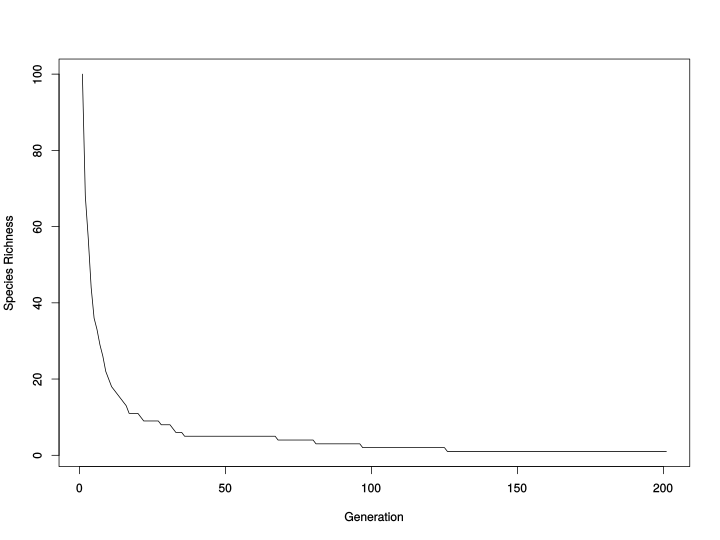
\includegraphics[width = \textwidth]{../Results/question_8.pdf}
			\caption{Species richness moving to one when under Netural Theory simulation with no speciation}
		\end{figure}
			
			
		
		\subsection*{Question 12 - Neutral Time Series with Speciation}
			\begin{figure}[H]
				\begin{center}
				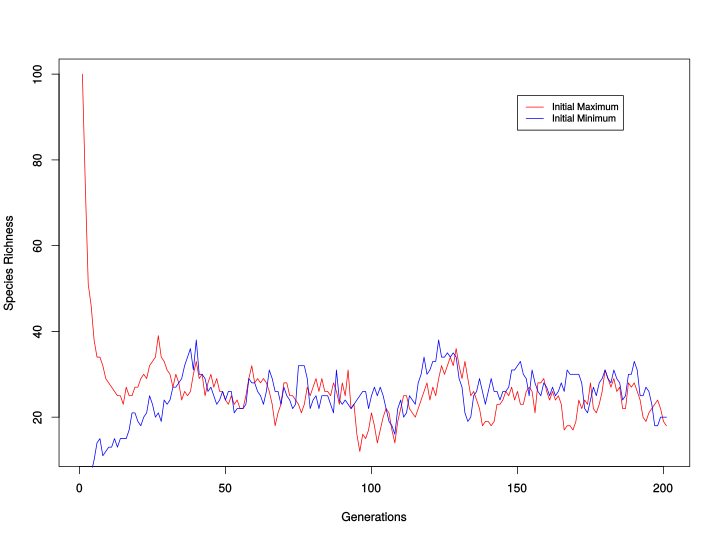
\includegraphics[width = \textwidth]{../Results/question_12.pdf}
				\caption{Spcecies richness under Neutral Theory simulation with 0.2 probability of speciation}
				\end{center}
			\end{figure}
			
			
		\subsection*{Question 16 - Species Abundances after Neutral Theory Simulation}
			\begin{figure}[H]
				\centering
				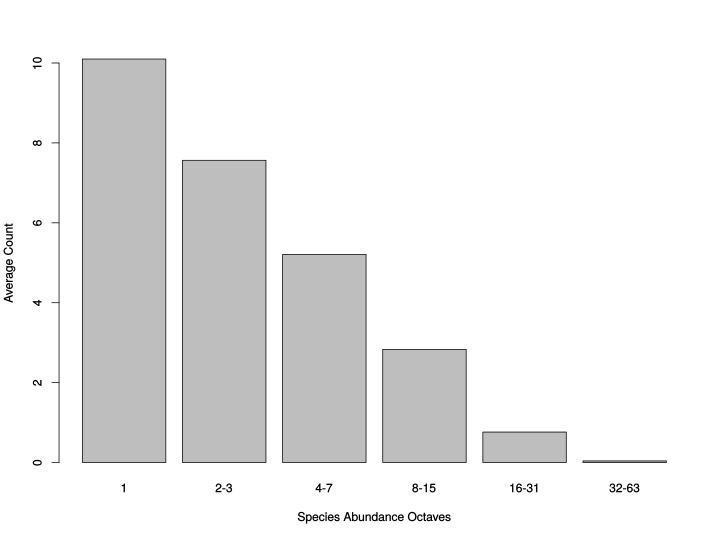
\includegraphics[width = \textwidth]{../Results/question_16.pdf}
				\caption{Distribution of Species Abundance after a Neutral Theory Simulation with speciation run for 2000 generation}
			\end{figure}
			
			
	\section*{Simulations Using HPC}
	
		\subsection*{Question 20 - Results from run on the Cluster}
			\begin{figure}[H]
				\centering
				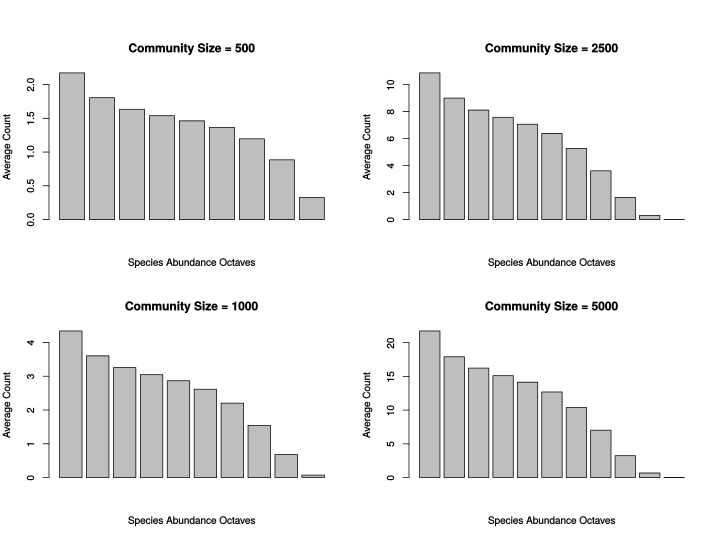
\includegraphics[width = \textwidth]{../Results/cluster_read.pdf}
				\caption{Distribution of mean Species Abundance's after Neutral Theory simulations with spciation run on four different community sizes}
			\end{figure}
					

			
		\subsection*{Challenge Question C - Species Richness by Generation}
			\begin{figure}[H]
				\centering
				\includegraphics[width = \textwidth]{../Results/challenge_c.pdf}
				\caption{Average species richness for the burn in period of each community size}
			\end{figure}
					

	\section*{Fractals in Nature}
	
		\subsection*{Fractal Dimensions}	
		
		\subsection*{The Chaos Game - Sierpinski Triangle}
			\begin{figure}[H]
				\centering
				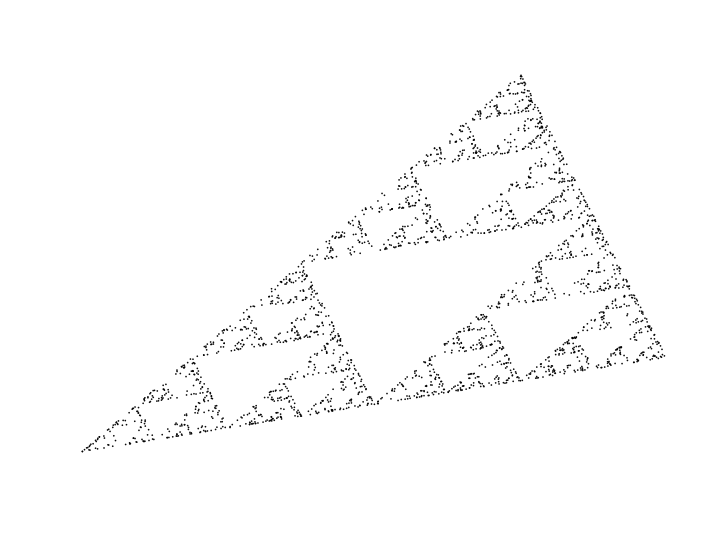
\includegraphics[width = \textwidth]{../Results/chaos_game.pdf}
				\caption{Sierpinski Triangle drawn between the points: (0,0), (3,4) and (4,1)}
			\end{figure}
					
		
		\subsection*{Challenge Question E - Sierpinski Triangle}
			\begin{figure}[H]
				\centering
				\includegraphics[width = \textwidth]{../Results/challenge_e.pdf}
				\caption{Sierpinski Triangle drawn between the points: (0,0), (4,0) and (2,$\sqrt{12}$) to make an equilateral triangle}
			\end{figure}
					
			
		\subsection*{Question 22 - Spiral}
		
		\subsection*{Question 23 - Spiral2}
			\begin{figure}[H]
				\centering
				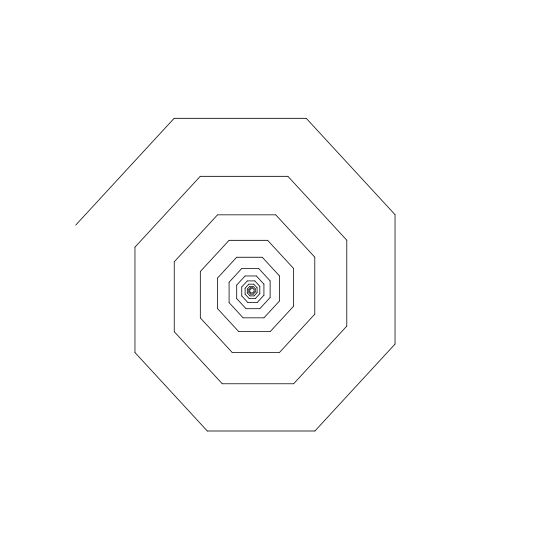
\includegraphics[width = \textwidth]{../Results/spiral_2.pdf}
				\caption{Spiral drawnby adding lines at $\pi/4$ radians and 0.95 length until lines went below a threshold length}
			\end{figure}
		
			
		\subsection*{Question 24 - Tree}
			\begin{figure}[H]
				\centering
				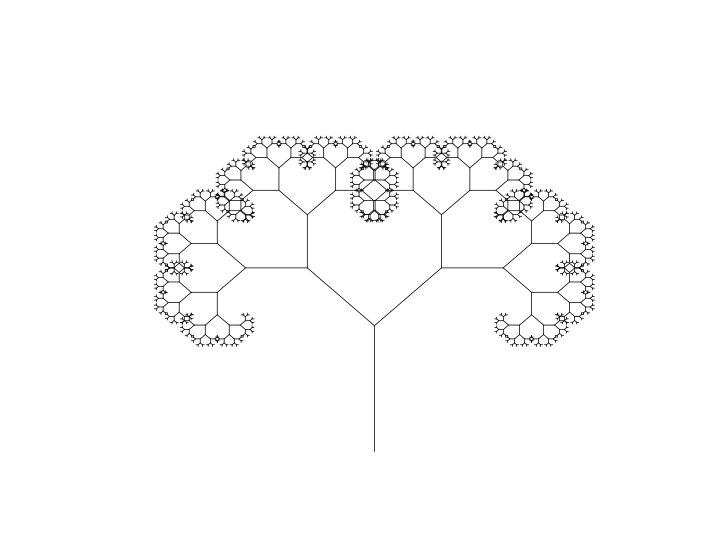
\includegraphics[width = \textwidth]{../Results/tree.pdf}
				\caption{Words Words Words}
			\end{figure}
			
			
		\subsection*{Quesiton 26 - Fern2}
			\begin{figure}[H]
				\centering
				\includegraphics[width = \textwidth]{../Results/fern_2.pdf}
				\caption{Words Words Words}
			\end{figure}
			
			
		\subsection*{Challenge Question F}
			\begin{figure}[H]
				\centering
				\includegraphics[width = \textwidth]{../Results/challenge_F1.pdf}
				\caption{Words Words Words}
			\end{figure}
			
			\begin{figure}[H]
				\centering
				
\includegraphics[width = \textwidth]{../Results/challenge_F2.pdf}
				\caption{Words Words Words}
			\end{figure}
					

	\end{flushleft}
\end{document}